\documentclass{standalone}
\usepackage{tikz}
\usetikzlibrary{patterns, positioning}

\begin{document}
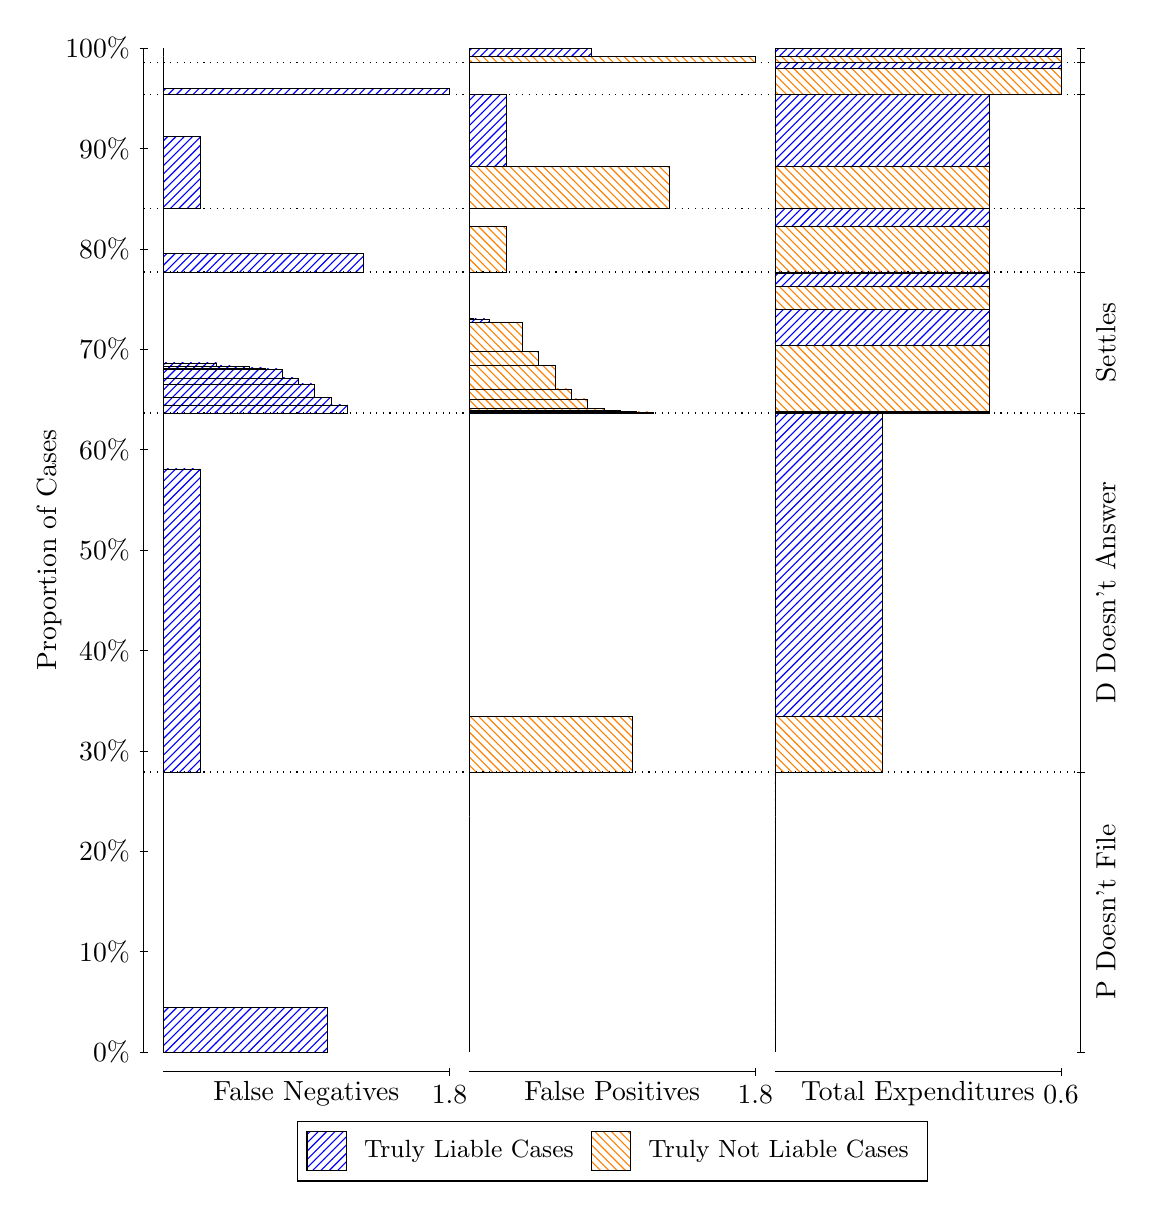
\begin{tikzpicture}
\draw[black, very thin] (1.5,1.75) -- (1.5,14.5);
\node[rotate=90, anchor=center] at (0.3, 8.125) {Proportion of Cases};
\draw[black, very thin] (1.45,1.75) -- (1.55,1.75);
\node[anchor=east] at (1.45, 1.75) {0\%};
\draw[black, very thin] (1.45,3.025) -- (1.55,3.025);
\node[anchor=east] at (1.45, 3.025) {10\%};
\draw[black, very thin] (1.45,4.3) -- (1.55,4.3);
\node[anchor=east] at (1.45, 4.3) {20\%};
\draw[black, very thin] (1.45,5.575) -- (1.55,5.575);
\node[anchor=east] at (1.45, 5.575) {30\%};
\draw[black, very thin] (1.45,6.85) -- (1.55,6.85);
\node[anchor=east] at (1.45, 6.85) {40\%};
\draw[black, very thin] (1.45,8.125) -- (1.55,8.125);
\node[anchor=east] at (1.45, 8.125) {50\%};
\draw[black, very thin] (1.45,9.4) -- (1.55,9.4);
\node[anchor=east] at (1.45, 9.4) {60\%};
\draw[black, very thin] (1.45,10.675) -- (1.55,10.675);
\node[anchor=east] at (1.45, 10.675) {70\%};
\draw[black, very thin] (1.45,11.95) -- (1.55,11.95);
\node[anchor=east] at (1.45, 11.95) {80\%};
\draw[black, very thin] (1.45,13.225) -- (1.55,13.225);
\node[anchor=east] at (1.45, 13.225) {90\%};
\draw[black, very thin] (1.45,14.5) -- (1.55,14.5);
\node[anchor=east] at (1.45, 14.5) {100\%};

\draw[black, very thin] (13.4,1.75) -- (13.4,14.5);
\draw[black, very thin] (13.35,1.75) -- (13.45,1.75);
\node[anchor=west] at (13.35, 1.75) {};
\draw[black, very thin] (13.35,5.306) -- (13.45,5.306);
\node[anchor=west] at (13.35, 5.306) {};
\draw[black, very thin] (13.35,9.8652) -- (13.45,9.8652);
\node[anchor=west] at (13.35, 9.8652) {};
\draw[black, very thin] (13.35,11.656) -- (13.45,11.656);
\node[anchor=west] at (13.35, 11.656) {};
\draw[black, very thin] (13.35,12.463) -- (13.45,12.463);
\node[anchor=west] at (13.35, 12.463) {};
\draw[black, very thin] (13.35,13.91) -- (13.45,13.91);
\node[anchor=west] at (13.35, 13.91) {};
\draw[black, very thin] (13.35,14.32) -- (13.45,14.32);
\node[anchor=west] at (13.35, 14.32) {};
\draw[black, very thin] (13.35,14.5) -- (13.45,14.5);
\node[anchor=west] at (13.35, 14.5) {};

\draw[black, very thin, pattern color=blue, pattern=north east lines] (1.75,1.75) rectangle (3.8262,2.3143);
\draw[black, very thin, pattern color=orange, pattern=north west lines] (1.75,2.3143) rectangle (1.75,5.306);
\draw[black, very thin, pattern color=blue, pattern=north east lines] (1.75,5.306) rectangle (2.2171,9.1554);
\draw[black, very thin, pattern color=orange, pattern=north west lines] (1.75,9.1554) rectangle (1.75,9.8652);
\draw[black, very thin, pattern color=blue, pattern=north east lines] (1.75,9.8652) rectangle (4.0857,9.9671);
\draw[black, very thin, pattern color=blue, pattern=north east lines] (1.75,9.9671) rectangle (3.8781,10.067);
\draw[black, very thin, pattern color=blue, pattern=north east lines] (1.75,10.067) rectangle (3.6705,10.236);
\draw[black, very thin, pattern color=blue, pattern=north east lines] (1.75,10.236) rectangle (3.4629,10.311);
\draw[black, very thin, pattern color=blue, pattern=north east lines] (1.75,10.311) rectangle (3.2552,10.425);
\draw[black, very thin, pattern color=blue, pattern=north east lines] (1.75,10.425) rectangle (3.0476,10.438);
\draw[black, very thin, pattern color=blue, pattern=north east lines] (1.75,10.438) rectangle (2.84,10.454);
\draw[black, very thin, pattern color=blue, pattern=north east lines] (1.75,10.454) rectangle (2.6324,10.462);
\draw[black, very thin, pattern color=blue, pattern=north east lines] (1.75,10.462) rectangle (2.4248,10.501);
\draw[black, very thin, pattern color=orange, pattern=north west lines] (1.75,10.501) rectangle (1.75,11.656);
\draw[black, very thin, pattern color=blue, pattern=north east lines] (1.75,11.656) rectangle (4.2933,11.889);
\draw[black, very thin, pattern color=orange, pattern=north west lines] (1.75,11.889) rectangle (1.75,12.463);
\draw[black, very thin, pattern color=blue, pattern=north east lines] (1.75,12.463) rectangle (2.2171,13.374);
\draw[black, very thin, pattern color=orange, pattern=north west lines] (1.75,13.374) rectangle (1.75,13.91);
\draw[black, very thin, pattern color=blue, pattern=north east lines] (1.75,13.91) rectangle (5.3833,13.984);
\draw[black, very thin, pattern color=orange, pattern=north west lines] (1.75,13.984) rectangle (1.75,14.32);
\draw[black, very thin, pattern color=orange, pattern=north west lines] (1.75,14.32) rectangle (1.75,14.392);
\draw[black, very thin, pattern color=blue, pattern=north east lines] (1.75,14.392) rectangle (1.75,14.5);
\draw[black, very thin, pattern color=orange, pattern=north west lines] (5.6333,1.75) rectangle (5.6333,4.7417);
\draw[black, very thin, pattern color=blue, pattern=north east lines] (5.6333,4.7417) rectangle (5.6333,5.306);
\draw[black, very thin, pattern color=orange, pattern=north west lines] (5.6333,5.306) rectangle (7.7095,6.0158);
\draw[black, very thin, pattern color=blue, pattern=north east lines] (5.6333,6.0158) rectangle (5.6333,9.8652);
\draw[black, very thin, pattern color=orange, pattern=north west lines] (5.6333,9.8652) rectangle (7.969,9.8789);
\draw[black, very thin, pattern color=orange, pattern=north west lines] (5.6333,9.8789) rectangle (7.7614,9.8855);
\draw[black, very thin, pattern color=orange, pattern=north west lines] (5.6333,9.8855) rectangle (7.5538,9.9004);
\draw[black, very thin, pattern color=orange, pattern=north west lines] (5.6333,9.9004) rectangle (7.3462,9.9193);
\draw[black, very thin, pattern color=orange, pattern=north west lines] (5.6333,9.9193) rectangle (7.1386,10.043);
\draw[black, very thin, pattern color=orange, pattern=north west lines] (5.6333,10.043) rectangle (6.931,10.171);
\draw[black, very thin, pattern color=orange, pattern=north west lines] (5.6333,10.171) rectangle (6.7233,10.466);
\draw[black, very thin, pattern color=orange, pattern=north west lines] (5.6333,10.466) rectangle (6.5157,10.651);
\draw[black, very thin, pattern color=orange, pattern=north west lines] (5.6333,10.651) rectangle (6.3081,11.02);
\draw[black, very thin, pattern color=blue, pattern=north east lines] (5.6333,11.02) rectangle (5.8929,11.06);
\draw[black, very thin, pattern color=blue, pattern=north east lines] (5.6333,11.06) rectangle (5.6852,11.067);
\draw[black, very thin, pattern color=blue, pattern=north east lines] (5.6333,11.067) rectangle (5.6333,11.656);
\draw[black, very thin, pattern color=orange, pattern=north west lines] (5.6333,11.656) rectangle (6.1005,12.231);
\draw[black, very thin, pattern color=blue, pattern=north east lines] (5.6333,12.231) rectangle (5.6333,12.463);
\draw[black, very thin, pattern color=orange, pattern=north west lines] (5.6333,12.463) rectangle (8.1767,12.999);
\draw[black, very thin, pattern color=blue, pattern=north east lines] (5.6333,12.999) rectangle (6.1005,13.91);
\draw[black, very thin, pattern color=orange, pattern=north west lines] (5.6333,13.91) rectangle (5.6333,14.246);
\draw[black, very thin, pattern color=blue, pattern=north east lines] (5.6333,14.246) rectangle (5.6333,14.32);
\draw[black, very thin, pattern color=orange, pattern=north west lines] (5.6333,14.32) rectangle (9.2667,14.392);
\draw[black, very thin, pattern color=blue, pattern=north east lines] (5.6333,14.392) rectangle (7.1905,14.5);
\draw[black, very thin, pattern color=orange, pattern=north west lines] (9.5167,1.75) rectangle (9.5167,4.7417);
\draw[black, very thin, pattern color=blue, pattern=north east lines] (9.5167,4.7417) rectangle (9.5167,5.306);
\draw[black, very thin, pattern color=orange, pattern=north west lines] (9.5167,5.306) rectangle (10.879,6.0158);
\draw[black, very thin, pattern color=blue, pattern=north east lines] (9.5167,6.0158) rectangle (10.879,9.8652);
\draw[black, very thin, pattern color=orange, pattern=north west lines] (9.5167,9.8652) rectangle (12.242,9.8786);
\draw[black, very thin, pattern color=blue, pattern=north east lines] (9.5167,9.8786) rectangle (12.242,9.8862);
\draw[black, very thin, pattern color=orange, pattern=north west lines] (9.5167,9.8862) rectangle (12.242,10.727);
\draw[black, very thin, pattern color=blue, pattern=north east lines] (9.5167,10.727) rectangle (12.242,11.178);
\draw[black, very thin, pattern color=orange, pattern=north west lines] (9.5167,11.178) rectangle (12.242,11.473);
\draw[black, very thin, pattern color=blue, pattern=north east lines] (9.5167,11.473) rectangle (12.242,11.642);
\draw[black, very thin, pattern color=orange, pattern=north west lines] (9.5167,11.642) rectangle (12.242,11.649);
\draw[black, very thin, pattern color=blue, pattern=north east lines] (9.5167,11.649) rectangle (12.242,11.656);
\draw[black, very thin, pattern color=orange, pattern=north west lines] (9.5167,11.656) rectangle (12.242,12.231);
\draw[black, very thin, pattern color=blue, pattern=north east lines] (9.5167,12.231) rectangle (12.242,12.463);
\draw[black, very thin, pattern color=orange, pattern=north west lines] (9.5167,12.463) rectangle (12.242,12.999);
\draw[black, very thin, pattern color=blue, pattern=north east lines] (9.5167,12.999) rectangle (12.242,13.91);
\draw[black, very thin, pattern color=orange, pattern=north west lines] (9.5167,13.91) rectangle (13.15,14.246);
\draw[black, very thin, pattern color=blue, pattern=north east lines] (9.5167,14.246) rectangle (13.15,14.32);
\draw[black, very thin, pattern color=orange, pattern=north west lines] (9.5167,14.32) rectangle (13.15,14.392);
\draw[black, very thin, pattern color=blue, pattern=north east lines] (9.5167,14.392) rectangle (13.15,14.5);
\draw[black, dotted] (1.5,5.306) -- (13.4,5.306);
\draw[black, dotted] (1.5,9.8652) -- (13.4,9.8652);
\draw[black, dotted] (1.5,11.656) -- (13.4,11.656);
\draw[black, dotted] (1.5,12.463) -- (13.4,12.463);
\draw[black, dotted] (1.5,13.91) -- (13.4,13.91);
\draw[black, dotted] (1.5,14.32) -- (13.4,14.32);
\draw[black, very thin] (1.75,1.5) -- (5.3833,1.5);
\node[anchor=north] at (3.5667, 1.5) {False Negatives};
\draw[black, very thin] (5.3833,1.45) -- (5.3833,1.55);
\node[anchor=north] at (5.3833, 1.45) {1.8};

\draw[black, very thin] (5.6333,1.5) -- (9.2667,1.5);
\node[anchor=north] at (7.45, 1.5) {False Positives};
\draw[black, very thin] (9.2667,1.45) -- (9.2667,1.55);
\node[anchor=north] at (9.2667, 1.45) {1.8};

\draw[black, very thin] (9.5167,1.5) -- (13.15,1.5);
\node[anchor=north] at (11.333, 1.5) {Total Expenditures};
\draw[black, very thin] (13.15,1.45) -- (13.15,1.55);
\node[anchor=north] at (13.15, 1.45) {0.6};

\node[black, centered, rotate=90] at (13.72, 3.528) {P Doesn't File};
\node[black, centered, rotate=90] at (13.72, 7.5856) {D Doesn't Answer};
\node[black, centered, rotate=90] at (13.72, 10.761) {Settles};





\draw (7.449999999999999,1.5) node[draw=none] (baseCoordinate) {};
\begin{scope}[align=center]
        \matrix[scale=0.5, draw=black, below=0.5cm of baseCoordinate, nodes={draw}, column sep=0.1cm]{
            \node[rectangle, draw, minimum width=0.5cm, minimum height=0.5cm, pattern=north east lines, pattern color=blue] {}; &
            \node[draw=none, font=\small] (B) {Truly Liable Cases}; &
            \node[rectangle, draw, minimum width=0.5cm, minimum height=0.5cm, pattern=north west lines, pattern color=orange] {}; &
            \node[draw=none, font=\small] (B) {Truly Not Liable Cases}; \\
            };
\end{scope}

\end{tikzpicture}
\end{document}